%             **********************************************************             %
%             Category Theory for Programmers by Bartosz Milewski                    %
%                                                                                    %
%             Compiled by Igal Tabachnik                                             %
%             https://github.com/hmemcpy/milewski-ctfp-pdf                           %
%                                                                                    %
%             This file is licensed under a Creative Commons                         %
%             Attribution-ShareAlike 4.0 International License                       %
%             (http://creativecommons.org/licenses/by-sa/4.0/).                      %
%             **********************************************************             %

% HISTORY:
% * Version 0.2 (October, 2017) - Math typesetting and lots of tweaks!
%
% * Version 0.1 (September, 2017) by Igal Tabachnik.
%   Based on the SICP PDF work of Andres Raba et al.
%   https://github.com/sarabander/sicp-pdf
%
%   Almost verbatim translation of the blog posts. Slight adjustments to images and text.

% !TEX TS-program = xelatex
% !TEX encoding = UTF-8 Unicode

\documentclass[11pt,oneside]{book}

% New line height: 1.05 * 1.2 = 1.26
\renewcommand{\baselinestretch}{1.05}

% Font settings
\usepackage{minted} %----------------------------------%  Note:
\usepackage[no-math]{fontspec}                         %  This exact order
\defaultfontfeatures{%                                 %  of declarations
  Scale=MatchLowercase, % needed here ...              %  is important for
}                                                      %  single quotes not
\setmonofont{Inconsolata LGC}                          %  to turn out curly
                                                       %  ("typographic")
\defaultfontfeatures{%                                 %  in verbatim blocks
  Scale=MatchLowercase, % ... and here again           %  of Haskell code.
  Mapping=tex-text,                                    %  Now the quote is
  SmallCapsFeatures={LetterSpace=2.5,WordSpace=1.05},  %  upright and safely
}                                                      %  copy-pasteable to
\setmainfont{Linux Libertine O}                        %  the REPL without
\setsansfont{Linux Biolinum O} %-----------------------%  giving errors.

% To use Libertine letters and numbers,
% but tx-style operators in math environment:
\usepackage[libertine]{newtxmath}
\usepackage{amsmath}
% Needed to display additional math unicode symbols (like double-colon)
\usepackage{unicode-math}
\setmathfont{Libertinus Math}

\usepackage[all]{nowidow}

% So that file names with multiple dots don't confuse
% graphicx package when using \includegraphics command:
\usepackage[multidot]{grffile}
\usepackage{graphicx}
\usepackage{caption, wrapfig, framed, subfigure}
\usepackage[export]{adjustbox}
\captionsetup{labelformat=empty,font=scriptsize}

\usepackage[usenames,dvipsnames,x11names]{xcolor}
\usepackage{longtable}
\usepackage{booktabs}
% Workaround to fix mismatched left and right math delimiters. Taken from:
% http://tex.stackexchange.com/questions/63410/parentheses-differ-xelatex-fontspec-newtxmath-libertine
\DeclareSymbolFont{parenthesis}{T1}{fxl}{m}{n}
\DeclareMathDelimiter{(}{\mathopen}{parenthesis}{"28}{largesymbols}{"00}
\DeclareMathDelimiter{)}{\mathclose}{parenthesis}{"29}{largesymbols}{"01}
\DeclareMathDelimiter{[}{\mathopen}{parenthesis}{"5B}{largesymbols}{"02}
\DeclareMathDelimiter{]}{\mathclose}{parenthesis}{"5D}{largesymbols}{"03}
\DeclareMathDelimiter{\lbrace}{\mathopen}{parenthesis}{"7B}{largesymbols}{"08}
\DeclareMathDelimiter{\rbrace}{\mathclose}{parenthesis}{"7D}{largesymbols}{"09}

\usepackage{fancyvrb}
\usepackage{imakeidx}
\usepackage[totoc,font=footnotesize]{idxlayout}
\usepackage{fancyhdr}
\pagestyle{plain}
\usepackage[final]{pdfpages} % inserts pages from a pdf file

% Page geometry for 10-inch tablets:
\usepackage[papersize={148mm,197mm},
            top=21mm,
            textwidth=111mm,  % increase one or both of these by 1mm or so to
            textheight=148mm, % make the source compile with TeX Live 2013
            hcentering,       % if you get "Too many unprocessed floats" error
]{geometry}

\usepackage{titlesec}  % to change the appearance of section titles
\usepackage{listings}  % for syntax highlighted code listings
\usepackage{verbatim}  % for simple verbatim and comment environments
\usepackage{enumerate} % allows customized labels in enumerations
\usepackage{enumitem}  % allows nested enumeration with numbers
\usepackage{hyperref}  % makes cross references and URLs clickable
\definecolor{LinkRed}{HTML}{80171F}
\hypersetup{
  pdfauthor={Bartosz Milewski},
  pdftitle={Category Theory for Programmers},
  pdfsubject={category theory, computer science, programming, abstraction},
  colorlinks=true,
  linkcolor=LinkRed,
  urlcolor=LinkRed,
}
\usepackage{subfiles}
\makeatletter
\let\org@subfile\subfile
\renewcommand*{\subfile}[1]{%
  \filename@parse{#1}% LaTeX's file name parser
  \expandafter
  \graphicspath\expandafter{\expandafter{\filename@area}}%
  \org@subfile{"#1"}%
}
\makeatother

% Document colors
\definecolor{SchemeLight}   {HTML} {686868}
\definecolor{SchemeSteel}   {HTML} {888888}
\definecolor{SchemeDark}    {HTML} {262626}
\definecolor{SchemeBlue}    {HTML} {4172A3}
\definecolor{SchemeGreen}   {HTML} {487818}
\definecolor{SchemeBrown}   {HTML} {A07040}
\definecolor{SchemeRed}     {HTML} {AD4D3A}
\definecolor{SchemeViolet}  {HTML} {7040A0}
\definecolor{DropCapGray}   {HTML} {B8B8B8}
\definecolor{ChapterGray}   {HTML} {C8C8C8}
\definecolor{ChapterViolet} {HTML} {AEAECE}
\definecolor{DropCapViolet} {HTML} {9090C0}

\usepackage{lettrine}  % adds commands that make drop capitals
\renewcommand{\LettrineFontHook}{\rmfamily\mdseries\color{DropCapViolet}}
\renewcommand{\DefaultLraise}{0.00}
\renewcommand{\DefaultLoversize}{0.02}
\renewcommand{\DefaultLhang}{0.12}
\setlength{\DefaultFindent}{1pt}
\setlength{\DefaultNindent}{0em}

\renewcommand{\partname}{}
\renewcommand{\thepart}{}

\newcommand{\acronym}[1]{\textsc{\fontspec[Numbers={OldStyle}]{Linux Libertine O}\MakeLowercase{#1}}}
\newcommand{\newterm}[1]{\index{#1}\emph{#1}}
\newcommand{\code}[1]{\texttt{#1}}
\newcommand{\heading}[1]{{\sffamily\bfseries #1}}
\newcommand{\mono}[1]{\hbox{\ttfamily\scriptsize #1}}
\newcommand{\monoit}[1]{\hbox{\ttfamily\itshape\scriptsize #1}}
\newcommand{\mathtext}[1]{\ensuremath{\pmb{#1}}}
\newcommand{\urlref}[2]{\href{#1}{#2}\urlfootnote{#1}}

\makeatletter
\newcommand\urlfootnote@[1]{\footnote{\url@{#1}}}
\DeclareRobustCommand{\urlfootnote}{\hyper@normalise\urlfootnote@}
\makeatother

\titleformat{\chapter}[display]
  {\color{SchemeDark}\normalfont\sffamily\bfseries\LARGE}
  {\filright \color{ChapterViolet}\sffamily\mdseries
    \fontsize{6em}{0em}\selectfont
    \oldstylenums{\thechapter}}
  {1em}
  {\filright}

\titleformat{\section}
{\color{SchemeDark}\normalfont\Large\sffamily\bfseries}
{\color{DropCapViolet}\thesection}{0.8em}{}

\titleformat{\subsection}
{\color{SchemeDark}\normalfont\large\sffamily\bfseries}
{\color{DropCapViolet}\thesubsection}{0.8em}{}

\titleformat{\subsubsection}
{\color{black}\normalfont\normalsize\sffamily\bfseries}
{\color{DropCapViolet}\thesubsubsection}{0.8em}{}

\setcounter{secnumdepth}{3}
\setcounter{tocdepth}{3}

\frenchspacing
\makeindex

\providecommand{\tightlist}{%
\setlength{\itemsep}{0pt}\setlength{\parskip}{0pt}}

%====================%
%  End of preamble.  %
%====================%

\begin{document}
\newcommand{\cat}{%
\mathbf%
}
\newcommand{\idarrow}[1][]{%
\mathbf{id}_{#1}%
}
\newcommand{\Set}{\cat{Set}}
\newcommand{\Rel}{\cat{Rel}}
\newcommand{\Cat}{\cat{Cat}}
\newcommand{\id}{\mathbf{id}}

\newcommand{\stimes}{{\times}}

\frontmatter

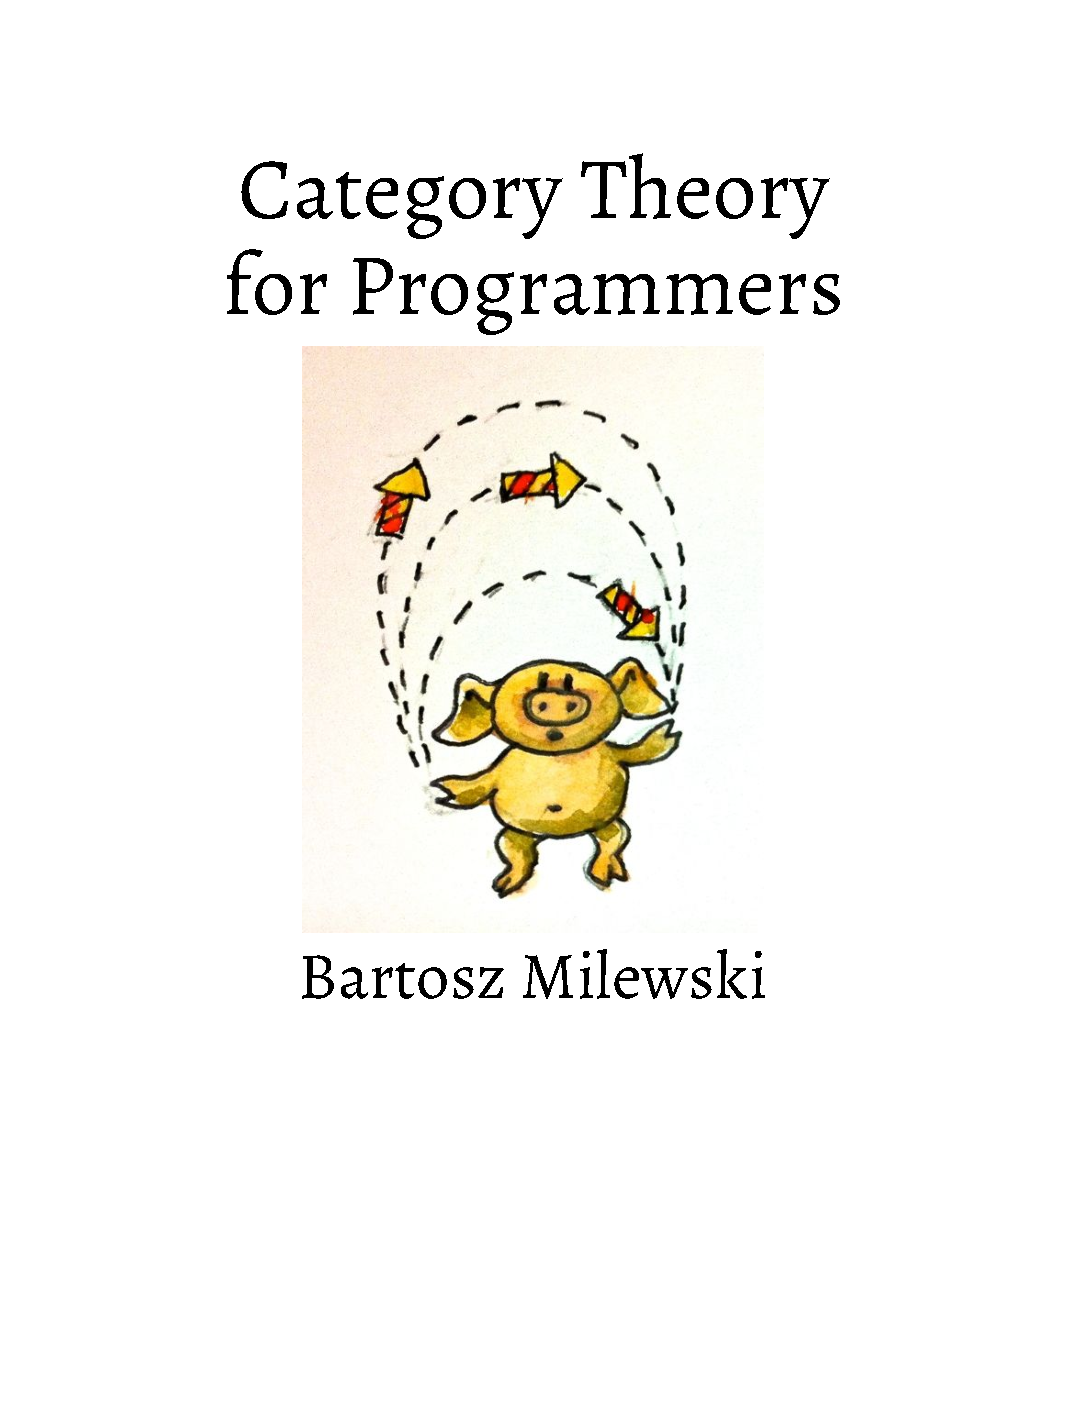
\includepdf[scale=0.92]{coverpage.pdf}

\pagebreak

\vspace*{\fill}
\thispagestyle{empty}

\begin{small}
\begin{center}

\noindent
Category Theory for Programmers\\

\vspace{1.0em}
\noindent
Bartosz Milewski\\

\vspace{1.26em}
\noindent
Version 0.2, October 2017\\

\vspace{1.6em}
\noindent

\includegraphics[width=3mm]{fig/icons/cc.pdf}

\includegraphics[width=3mm]{fig/icons/by.pdf}

\includegraphics[width=3mm]{fig/icons/sa.pdf}

\vspace{0.4em}
\noindent
This work is licensed under a Creative Commons\\
Attribution-ShareAlike 4.0 International License 
(\href{http://creativecommons.org/licenses/by-sa/4.0/}{\acronym{CC BY-SA 4.0}}).

\vspace{1.26em}
\noindent
Converted to \LaTeX{} from a series of blog posts by \href{https://bartoszmilewski.com/2014/10/28/category-theory-for-programmers-the-preface/}{Bartosz Milewski}.\\
PDF compiled by \href{https://github.com/hmemcpy/milewski-ctfp-pdf}{Igal Tabachnik}.\\

\end{center}
\end{small}

\pagebreak
\tableofcontents

\chapter*{Preface}
\addcontentsline{toc}{chapter}{Preface}
\label{Preface}

\subfile{content/0.0/Preface}

\mainmatter

\part{Part One}

\chapter{Category: The Essence of Composition}\label{category-the-essence-of-composition}
\subfile{content/1.1/Category - The Essence of Composition}

\chapter{Types and Functions}\label{types-and-functions}
\subfile{content/1.2/Types and Functions}

\chapter{Categories Great and Small}\label{categories-great-and-small}
\subfile{content/1.3/Categories Great and Small}

\chapter{Kleisli Categories}\label{kleisli-categories-page}
\subfile{content/1.4/Kleisli Categories}

\chapter{Products and Coproducts}\label{products-and-coproducts}
\subfile{content/1.5/Products and Coproducts}

\chapter{Simple Algebraic Data Types}\label{simple-algebraic-data-types}
\subfile{content/1.6/Simple Algebraic Data Types}

\chapter{Functors}\label{functors}
\subfile{content/1.7/Functors}

\chapter{Functoriality}\label{functoriality}
\subfile{content/1.8/Functoriality}

\chapter{Function Types}\label{function-types}
\subfile{content/1.9/Function Types}

\chapter{Natural Transformations}\label{natural-transformations}
\subfile{content/1.10/Natural Transformations}

\part{Part Two}

\chapter{Declarative Programming}\label{declarative-programming}
\subfile{content/2.1/Declarative Programming}

\chapter{Limits and Colimits}\label{limits-and-colimits}
\subfile{content/2.2/Limits and Colimits}

\chapter{Free Monoids}\label{free-monoids}
\subfile{content/2.3/Free Monoids}

\chapter{Representable Functors}\label{representable-functors}
\subfile{content/2.4/Representable Functors}

\chapter{The Yoneda Lemma}\label{the-yoneda-lemma}
\subfile{content/2.5/The Yoneda Lemma}

\chapter{Yoneda Embedding}\label{yoneda-embedding}
\subfile{content/2.6/Yoneda Embedding}

\part{Part Three}

\chapter{It's All About Morphisms}
\subfile{content/3.1/It's All About Morphisms}

\chapter{Adjunctions}\label{adjunctions}
\subfile{content/3.2/Adjunctions}

\chapter{Free/Forgetful Adjunctions}\label{free-forgetful-adjunctions}
\subfile{content/3.3/Free-Forgetful Adjunctions}

\chapter{Monads: Programmer's Definition}\label{monads-programmers-definition}
\subfile{content/3.4/Monads - Programmer's Definition}

\chapter{Monads and Effects}\label{monads-and-effects}
\subfile{content/3.5/Monads and Effects}

\chapter{Monads Categorically}\label{monads-categorically}
\subfile{content/3.6/Monads Categorically}

\chapter{Comonads}\label{comonads}
\subfile{content/3.7/Comonads}

\chapter{F-Algebras}\label{f-algebras}
\subfile{content/3.8/F-Algebras}

\chapter{Algebras for Monads}\label{algebras-for-monads}
\subfile{content/3.9/Algebras for Monads}

\chapter{Ends and Coends}\label{ends-and-coends}
\subfile{content/3.10/Ends and Coends}

\chapter{Kan Extensions}\label{kan-extensions}
\subfile{content/3.11/Kan Extensions}

\chapter{Enriched Categories}\label{enriched-categories}
\subfile{content/3.12/Enriched Categories}

\chapter{Topoi}\label{topoi}
\subfile{content/3.13/Topoi}

\chapter{Lawvere Theories}\label{lawvere-theories}
\subfile{content/3.14/Lawvere Theories}

\chapter{Monads, Monoids, and Categories}\label{monads-monoids-categories}
\subfile{content/3.15/Monads, Monoids, and Categories}

\backmatter

\chapter*{Acknowledgments}
\addcontentsline{toc}{chapter}{Acknowledgments}

\noindent
I’d like to thank Edward Kmett and Gershom Bazerman for checking my math
and logic, and André van Meulebrouck, who has been volunteering his editing
help throughout this series of posts.

\vspace{1.0em}
\noindent
I’d like to thank Andrew Su on for rewriting my C++ monoid concept
code according to his and Bjarne Stroustrup’s latest proposal.

\vspace{1.0em}
\noindent
I'm grateful to Eric Niebler for reading the draft and providing the
clever implementation of \code{compose} that uses advanced features of
C++14 to drive type inference. I was able to cut the whole section of
old fashioned template magic that did the same thing using type traits.
Good riddance! I'm also grateful to Gershom Bazerman for useful comments
that helped me clarify some important points.

\setindexprenote{\normalsize
\begin{quote} Any inaccuracies in this index may be explained by the fact
that it has been prepared with the help of a computer.

---Donald E. Knuth, \textit{Fundamental Algorithms}\\
(Volume 1 of \textit{The Art of Computer Programming})
\end{quote}}

\printindex

\chapter*{Colophon}
\addcontentsline{toc}{chapter}{Colophon}
\lettrine[lraise=-0.03,loversize=0.08]{T}{his book} was compiled by converting the original text by Bartosz Milewski into \LaTeX{} format, by
first scraping the original WordPress blog posts using Mercury Web Parser\urlfootnote{https://mercury.postlight.com/web-parser/}
to get a clean HTML content, modifying and tweaking with Beautiful Soup\urlfootnote{https://www.crummy.com/software/BeautifulSoup/}, finally, converting to LaTeX with Pandoc\urlfootnote{https://pandoc.org/}.

The typefaces are Linux Libertine for body text and Linux Biolinum for headings, both by Philipp H. Poll. Typewriter face is Inconsolata
created by Raph Levien and supplemented by Dimosthenis Kaponis and Takashi Tanigawa in the form of Inconsolata \acronym{LGC}. The cover page
typeface is Alegreya, designed by Juan Pablo del Peral.

Graphic design and typography are done by Andres Raba. Diagrams are drawn with Inkscape.

\chapter*{Copyleft notice}
\addcontentsline{toc}{chapter}{Copyleft notice}
\lettrine[lraise=-0.03,loversize=0.08]{T}{his book} is \textbf{Libre} and follows the philosophy of Free Software\urlfootnote{https://www.gnu.org/philosophy/free-sw.en.html}: 
you can use this book as you like, the source is available, you can redistribute
this book and you can distribute your own version. That means you can print it,
photocopy it, e-mail it, upload it to websites, change it, translate it, remix it, delete bits,
and draw all over it.

This book is Copyleft: if you change the book and distribute your own version, you must also pass these freedoms to its recipients.
This book uses the Creative Commons Attribution-ShareAlike 4.0 International License 
(\href{http://creativecommons.org/licenses/by-sa/4.0/}{\acronym{CC BY-SA 4.0}}).


\end{document}
